\documentclass[12pt,a4paper]{article}

\usepackage[UTF8]{ctex}
\usepackage[scale=0.8]{geometry}
\usepackage{latexsym,amsmath,amsfonts,amssymb,mathrsfs,bm}
\usepackage{abstract,appendix,titlesec,titletoc}
\usepackage{diagbox,booktabs,longtable,tabularx}
\usepackage[amsmath,thmmarks,hyperref]{ntheorem}
\usepackage{fancyhdr,indentfirst}
\usepackage[colorlinks=true]{hyperref}
\usepackage{makeidx,cleveref}
\usepackage[sort&compress, numbers]{natbib}
\usepackage{graphicx,epsfig,subfig}
\usepackage{algorithm,algorithmic}
\usepackage{xcolor}

%\setlength{\lineskip}{\baselineskip}
\setlength{\parskip}{0.5\baselineskip}

\title{稀疏拟牛顿迭代法}
\author{sis-flag}
\date{\today}

\begin{document}

\maketitle

求解非线性方程组时,常用的方法有不动点迭代,Newton迭代和Broyden迭代。不动点迭代构造方法和计算都很简单,但收敛较慢。Newton迭代收敛较快,但是需要方程的导数信息。Broyden迭代用函数值重构导数信息,但是对于方程维数很高的情况,计算其中的Jacobi矩阵很耗时。注意到在微分方程数值解的格式中,很多矩阵都具有稀疏性。因此我们希望利用稀疏性重构导数信息,设计更快速的迭代求解方法。

这里介绍各种的非线性迭代方法,同时提出我们的新想法。

\subsection*{以一维非线性方程为例}

我们先看一个简单的例子。

区域$\Omega = [0, 1]$。求解非线性椭圆方程
\begin{align*}
- & (a(x, u) \; u'(x))' = f(x, u) \qquad x \in \Omega \\
& u(0) = g_0 \quad u(1) = g_1
\end{align*}

\textbf{方程要满足存在唯一解,以及各种适定性。}由于我不知道PDE里面的结论,这里就先不写了。

\subsection*{数值格式}

均匀网格,步长是$h$。在网格上离散方程。定义流量$\bar{F}(x) = a(x, u(x)) \; u'(x)$,以下这些都是二阶近似
\begin{align*}
\bar{F}'(x_{k}) & \approx \frac{1}{h} (F(x_{k+1/2}) - F(x_{k-1/2})) \\
u'(x_{k+1/2}) & \approx \frac{1}{h} (u_{k+1} - u_{k}) \\
u(x_{k+1/2}) & \approx \frac{1}{2} (u_{k+1} + u_{k})
\end{align*}

最终的数值格式为
\begin{align*}
a_{k+1/2}(u_{k+1/2}) \; (u_{k} - u_{k+1}) + a_{k-1/2}(u_{k-1/2}) \; (u_{k} - u_{k-1}) = h^2 f_{k}(u_{k})
\end{align*}
边界条件$u_0 = g_0, u_N = g_1$。

其中$a(x_{k+1/2}, u)$简写成$a_{k+1/2}(u)$,$\frac{u_{k+1} + u_{k}}{2}$简写成$u_{k+1/2}$。其它符号类似。

写成矩阵的形式就是$A(u) u = F(u)$。其中
\begin{align*}
A_{k,k}(u) &= a_{k-1/2}(u_{k-1/2}) + a_{k+1/2}(u_{k+1/2}) \\
A_{k,k+1}(u) &= A_{k+1,k}(u) = -a_{k+1/2}(u_{k+1/2})
\end{align*}
右端项表示为
\begin{align*}
F_{1}(u) &= h^2 \; f_1(u_1) + a_{1/2} \; u_0 \\
F_{k}(u) &= h^2 \; f_{k}(u_{k}) \\
F_{N-1}(u) &= h^2 \; f_{N-1}(u_{N-1}) + a_{N-1/2} \; u_N
\end{align*}

\subsection*{非线性方程组}

求解数值格式,就是求解非线性方程组$\phi(u) = A(u) u - F(u) = 0$。这里的
\begin{align*}
\phi_{k}(u) = a_{k+1/2}(u_{k+1/2}) \; (u_{k} - u_{k+1}) + a_{k-1/2}(u_{k-1/2}) \; (u_{k} - u_{k-1}) - h^2 f_{k}(u_{k})
\end{align*}

显然$\phi_{k}$只和附近的$u_{k+1}, u_{k}, u_{k-1}$有关。

数值格式两边求导得到,非线性函数$\phi$的Jacobi矩阵$J(u)$为
\begin{align*}
J_{k,k}(u) = \frac{\partial \phi_{k}}{\partial u_{k}} & = \frac12 \; a_{k+1/2}'(u_{k+1/2}) \; (u_{k} - u_{k+1}) + a_{k+1/2}(u_{k+1/2}) \\
& + \frac12 \; a_{k-1/2}'(u_{k-1/2}) \; (u_{k} - u_{k-1}) + a_{k-1/2}(u_{k-1/2}) \\
& - h^2 \; f_{k}'(u_{k}) \\
J_{k,k+1}(u) = \frac{\partial \phi_{k}}{\partial u_{k+1}} & = \frac12 \; a_{k+1/2}'(u_{k+1/2}) \; (u_{k} - u_{k+1}) - a_{k+1/2}(u_{k+1/2}) \\
J_{k,k-1}(u) = \frac{\partial \phi_{k}}{\partial u_{k-1}} & = \frac12 \; a_{k-1/2}'(u_{k-1/2}) \; (u_{k} - u_{k-1}) - a_{k-1/2}(u_{k-1/2})
\end{align*}

注意观察导数
$$ J_{k,k+1} = \frac12 \; a_{k+1/2}'(u_{k+1/2}) \; {\color{red} (u_{k} - u_{k+1})} - a_{k+1/2}(u_{k+1/2}) $$
但是
$$ J_{k+1,k} = \frac12 \; a_{k+1/2}'(u_{k+1/2}) \; {\color{red} (u_{k+1} - u_{k})} - a_{k+1/2}(u_{k+1/2}) $$
所以对应的Jacobi矩阵$J(u)$不是对称矩阵。

\subsection*{Picard迭代法}

Picard迭代法直接用上一迭代步的$u^{(s)}$构建矩阵$A(u^{(s)})$,之后求解线性方程组。
\begin{align*}
u^{(s+1)} = {A(u^{(s)})}^{-1} \; F(u^{(s)})
\end{align*}
也就是
\begin{align*}
u^{(s+1)} = u^{(s)} - {A(u^{(s)})}^{-1} \; \phi(u^{(s)})
\end{align*}

从另一种角度看,它相当于在Newton迭代中用$A(u^{(s)})$近似导数矩阵,只不过近似的不是很好。

\subsection*{稳定化Picard迭代法*}

在抛物方程中,在时间步长充分小的条件下,Picard迭代可以证是压缩映射,收敛性可以保证。但是在椭圆方程中,Picard迭代并没有收敛性保证。实际的数值实验中,也可以观察到误差不是严格下降的。

注意到椭圆方程的解相当于抛物方程中时间趋于无穷时的解,我们可以把时间步偷偷加到非线性迭代中去,在论文中对外宣称是加了一个“稳定化”项,然后把内循环和外循环混淆起来,让时间步和Picard迭代同时进行,应该就可以构造出一个专门针对椭圆方程的,保证收敛的迭代方法。不过估计这种方法会比Picard迭代还要慢。

\subsection*{直接Newton迭代法}

从数值格式出发,在已知$J(u)$的情况下,可以得到牛顿迭代为
\begin{align*}
J(u^{(s)}) \; (u^{(s)} - u^{(s+1)}) = \phi(u^{(s)})
\end{align*}
也就是
\begin{align*}
u^{(s+1)} = u^{(s)} - (J(u^{(s)}))^{-1} \; \phi(u^{(s)})
\end{align*}

在这个例子中,$J(u)$是一个三对角矩阵,它在求解方程组时的运算量和Picard迭代是相同的。
如果把$J(u)$中所有和$a(x,u)$导数有关的项抹掉,$J(u)$就退化成为了$A(u)$,它就变成了Picard迭代。

\subsection*{Picard-Newton迭代法}

\subsection*{拟Newton迭代法(Broyden方法)}

\subsection*{JFNK迭代法}

\textbf{通过推导我们可以看出,导数矩阵一定是三对角的,也就是说矩阵的某些位置确定为0,这一点非常重要,前面提到的方法都没有考虑这一点。}

\subsection*{考虑稀疏性的Newton迭代法*}

\subsection*{考虑稀疏性的Broyden方法*}

用三对角矩阵$J^{(s)}$近似$J(u^{(s)})$,得到拟牛顿迭代为
\begin{align*}
J^{(s)} \; (u^{(s)} - u^{(s+1)}) = \phi(u^{(s)})
\end{align*}
其中$J^{(s)}$应满足割线的性质,也就是
\begin{align*}
J^{(s+1)} \; (u^{(s+1)} - u^{(s)}) = \phi(u^{(s+1)}) - \phi(u^{(s)}) \qquad J^{(s+1)} \; \Delta u^{(s)} = \Delta \phi^{(s)}
\end{align*}
下一步的导数可以看作是由上一步修正而来。

仅通过割线的性质是无法确定$\Delta J^{(s)}$的,在Broyden拟牛顿迭代中,要求$\Delta J^{(s)}$的秩为1,下面我们从另一个角度分析一下这样做的原因。

(分析略)

通过分析,Broyden方法相当于在保证割线$J^{(s+1)} \; \Delta u^{(s)} = \Delta \phi^{(s)}$的条件下,找距离原视矩阵最近的那个做为新的导数矩阵近似。

这样我们就可以把稀疏性条件加入到迭代中了。我们希望修正量在满足三对角的条件下,尽可能小。也就是
\begin{align*}
J^{(s+1)} = \arg \min \ \|J - J^{(s)}\|_F \quad \text{s.t.} \quad J^{(s+1)} \; \Delta u^{(s)} = \Delta \phi^{(s)} \qquad \Delta J^{(s+1)} \ \text{is spase}
\end{align*}

具体求解的过程中,定义$r^{(s)} = \phi^{(s)} - J^{(s)} - A^{(s)} + A^{(s+1)} \Delta u^{(s)}$。考虑方程的第$i$行
\begin{align*}
\Delta J^{(s)}_{i,i-1} \; \Delta u^{(s)}_{i-1} + \Delta J^{(s)}_{i,i} \; \Delta u^{(s)}_{i} + \Delta J^{(s)}_{i,i+1} \; \Delta u^{(s)}_{i+1} = r^{(s+1)}_{i}
\end{align*}
问题就转化成了求上面这个方程最靠近原点的解。解一定和平面的法向量同向,也就是
\begin{align*}
\Delta J^{(s)}_{i,j} = \frac{\Delta u^{(s)}_{j} \; r^{(s+1)}_{i}}{\sum_{j=i-1}^{i+1} (\Delta u^{(s)}_{j})^2} \quad j = i-1,i,i+1
\end{align*}

\subsection*{考虑稀疏性的拟牛顿迭代*}

同样用三对角矩阵$J^{(s)}$近似$\nabla \phi(u^{(s)})$,得到拟牛顿迭代为
\begin{align*}
J^{(s)} \; (u^{(s)} - u^{(s+1)}) = \phi(u^{(s)})
\end{align*}
其中$J^{(s)}$应满足割线的性质,也就是
\begin{align*}
J^{(s+1)} \; (u^{(s+1)} - u^{(s)}) = \phi(u^{(s+1)}) - \phi(u^{(s)}) \qquad J^{(s+1)} \; \Delta u^{(s)} = \Delta \phi^{(s)}
\end{align*}
仅仅通过这一个条件无法唯一确定$J^{(s+1)}$,因此我们需要多考虑几步的约束。也就是
\begin{align*}
J^{(s+1)} \; \Delta u^{(s-m)} = \Delta \phi^{(s-m)}, \quad m = 0, 1, \cdots N_D-1
\end{align*}
其中$N_D$是矩阵每一行最多的非零元个数,$J$每行有多少非零元,我们就需要多少个方程去约束它。

在这个例子中,$J$每行最多三个元素非零,而且它们的位置都已知。考虑矩阵的第$i$行,我们可以得到
\begin{align*}
\left[
\begin{array}{ccc}
\Delta u^{(s-2)}_{i-1} & \Delta u^{(s-1)}_{i-1} & \Delta u^{(s)}_{i-1} \\
\Delta u^{(s-2)}_{i} & \Delta u^{(s-1)}_{i} & \Delta u^{(s)}_{i} \\
\Delta u^{(s-2)}_{i+1} & \Delta u^{(s-1)}_{i+1} & \Delta u^{(s)}_{i+1} \\
\end{array}
\right]
\left[
\begin{array}{c}
J^{(s+1)}_{i,i-1} \\
J^{(s+1)}_{i,i} \\
J^{(s+1)}_{i,i+1} \\
\end{array}
\right]
=
\left[
\begin{array}{c}
\Delta \phi^{(s)}_{i} \\
\Delta \phi^{(s-1)}_{i} \\
\Delta \phi^{(s-2)}_{i} \\
\end{array}
\right]
\end{align*}
在每个单元上求解上面这个方程组,就可以得到每一步的矩阵$J$。

这里需要我们做出权衡,想要让方程组的解尽量逼近导数,就要$\Delta u^{(s)}$尽量小,但是如果$\Delta u^{(s)}$太小,就会造成矩阵近似奇异,增加舍入误差。
因此这里我们先用Picard迭代,迭代到$\|\phi(u^{(s)})\| < 10^{-2}$时,我们就认为迭代已经开始收敛,此时再用SQN方法加速。

\newpage
\subsection*{数值实验}

\textbf{由于Picard迭代抹去了扩散系数对$u$的导数,对于导数很大的情况,Picard迭代的效率就会慢。我们可以针对这一点设计算例。}

实验中
\begin{align*}
u(x) = \sin \pi x^2 \quad a(x,u) = \epsilon + u^2
\end{align*}
通过符号求导得到
\begin{align*}
f(x) & = 4 \, x^2 \, \pi ^2 \, \sin \left( \pi \, x^2 \right) \, \left( {\sin \left( \pi \, x^2 \right)}^2 + \epsilon \right) \\
& - 8 \, x^2 \, \pi^2 \, {\cos \left( \pi \, x^2 \right)}^2 \, \sin \left( \pi \, x^2 \right) \\
& - 2 \, \pi \, \cos \left( \pi \, x^2 \right) \, \left( {\sin \left( \pi \, x^2 \right)}^2 + \epsilon \right)
\end{align*}

选取$\epsilon = 1$,在不同的步长下用前文提到的格式求解,得到结果如下表\cref{t1}。

\begin{table}[h]
\centering
\begin{tabular}{c|cccc}
\hline
h & Picard & Newton & SQN2 & SQN1 \\
\hline
1/5 & 20 & 5 & 12 & 11 \\
1/20 & 15 & 5 & 13 & 13 \\
1/100 & 12 & 5 & 13 & 15 \\
\hline
\end{tabular}
\caption{迭代步数}
\label{t1}
\end{table}
我也不知道为什么迭代步数随网格变化这么大。但是这东西至少在大多数情况下不会比picard迭代更差。

选取$\epsilon = 0.01, h = 1/100$,这时Picard迭代就显示出了劣势。误差随迭代步数下降如图\cref{f1}。Picard用58步,SQN2用23步,Newton用14步。

\begin{figure}[h]
\centering
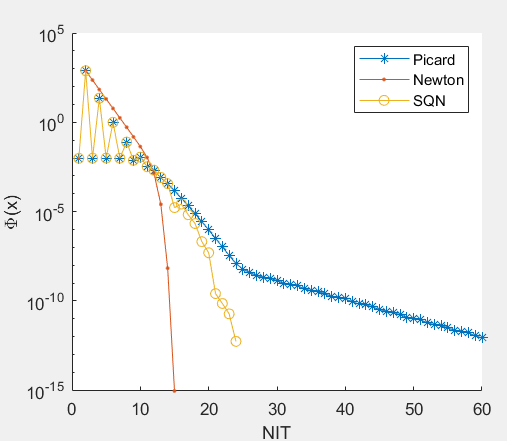
\includegraphics[width=0.5\linewidth]{1}
\caption{}
\label{f1}
\end{figure}




\end{document}